\subsection{Einregeln der optimalen Verzögerungszeit}
Da die Leitungen von den SEV zur Koinzidenzschaltung nicht zwingend gleich schnell sind, wird die Verzögerung zwischen den beiden Seiten optimiert.
Die Verzögerungszeit kann in beiden Leitungen separat erhöht werden, indem Kabel mit definierten Verzögerungen zugeschaltet werden.
Eine Verzögerung bei der einen Kabelleitung bewirkt eine relative 'Beschleunigung' der anderen Kabelleitung.
Die Zählrate $N$ wird in Abhängigkeit verschiedener Verzögerungszeiten $T_{\text{VZ}}$ gemessen (Tabelle \ref{tab:verzögerung}, Abbildung \ref{fig:verzögerung}).
\input{tabelleverzögerung.tex}
\begin{figure}[h!]
  \centering
  \includegraphics[width=\textwidth]{figverzögerung.pdf}
  \caption{Optimierung der Verzögerungszeit: Verzögerungszeit $T_{\text{VZ}}$ gegen die Zählrate $N$}
  \label{fig:verzögerung}
\end{figure}
Es wird eine Ausgleichsrechnung der Form
\begin{equation*}
  N = -a \left( T_{\text{VZ}} + \Delta T_{\text{VZ}} \right)^4+N_{\text{max}}
\end{equation*}
mit Python 3.6.3 vorgenommen.
Die Parameter ergeben sich zu
\begin{align*}
  a                     &=& \SI{  4.8215 \pm 0.2361 e32}{\frac{1}{s^4}}\\
  \Delta T_{\text{VZ}}  &=& \SI{  2.0854 \pm 0.2292 e-9}{s}\\
  N_{\text{max}}        &=& \SI{208.0012 \pm 3.5037 }{}.\\
\end{align*}
%die Parameter mit allen Nachkommastellen
%a     = -4.82149139e-04*1e36
%DTV   = 2.08543590*1e-9
%Nmax  = 208.001211
%da    = 2.36142749e-05*1e36
%dDTV  = 0.229205675*1e-9
%dNmax = 3.50366201
Dabei beschreibt $\Delta T_{\text{VZ}}$ die seitliche Verschiebung des Maximums und damit den Wert, der fortan als Verzögerung der Leitung gewählt wird.
Damit sind die Signale aus den SEV annähernd gleichzeitig an der Koinzidenzschaltung. $N_{\text{max}}$ ist die berechete maximale Zählrate.\\
Desweiteren wird die Halbwertsbreite der Zählrate bestimmt.
Die Halbwertsbreite ist im Diagramm durch eine Konstante bei $\frac{N_{\text{max}}}{2}=\SI{104.0006}{}$ dargestellt.
Die Halbwertsbreite wird als
\begin{equation*}
  w_{\text{N/2}}= \SI{42.7e-9}{s}
\end{equation*}
genähert.
\FloatBarrier
\subsection{Kalibrierung des Multi-Channel-Analysers}
Um vom Channel des Multi-Channel-Analysers auf die zugehörige Zeit zwischen den Impulsen schließen zu können, wird der Multi-Channel-Analyser kalibriert.
Die Channel werden in Abhängigkeit des zeitlichen Abstands der Signale vom Doppelimpulsgenerator gemessen (Tabelle \ref{tab:kalibrierung}, Abbildung \ref{fig:kalibrierung}).
\begin{table}[h!]
  \centering
  \caption{Messdaten zu Kalibrierung des Multi-Channel-Analysers}
  \label{tab:kalibrierung}
  \begin{tabular}{c c c c}
    \toprule
%    \multicolumn{3}{c}{$f_{\text{1, theo}}=\SI{0.1}{m}$} & \multicolumn{3}{c}{$f_{\text{2, theo}}=\SI{0.05}{m}$}\\
      Channel & $\Delta$ t $/ 10^{-6} s$ & Channel & $\Delta$ t $/ 10^{-6} s$ \\
      \midrule
         24   &   1407  &  247   &   1680 \\
         46   &   1561  &  270   &   1555 \\
         69   &   1400  &  292   &   1608 \\
         91   &   1294  &  315   &   1384 \\
        113   &   1298  &  337   &   1952 \\
        136   &   1034  &  359   &   1880 \\
        158   &   1502  &  382   &   2008 \\
        180   &   1336  &  404   &   2088 \\
        203   &   1700  &  427   &   2024 \\
        225   &   1644  &  445   &   3384 \\
    \bottomrule
  \end{tabular}
\end{table}

%\end{landscape}
%\end{document}

\begin{figure}[h!]
  \centering
  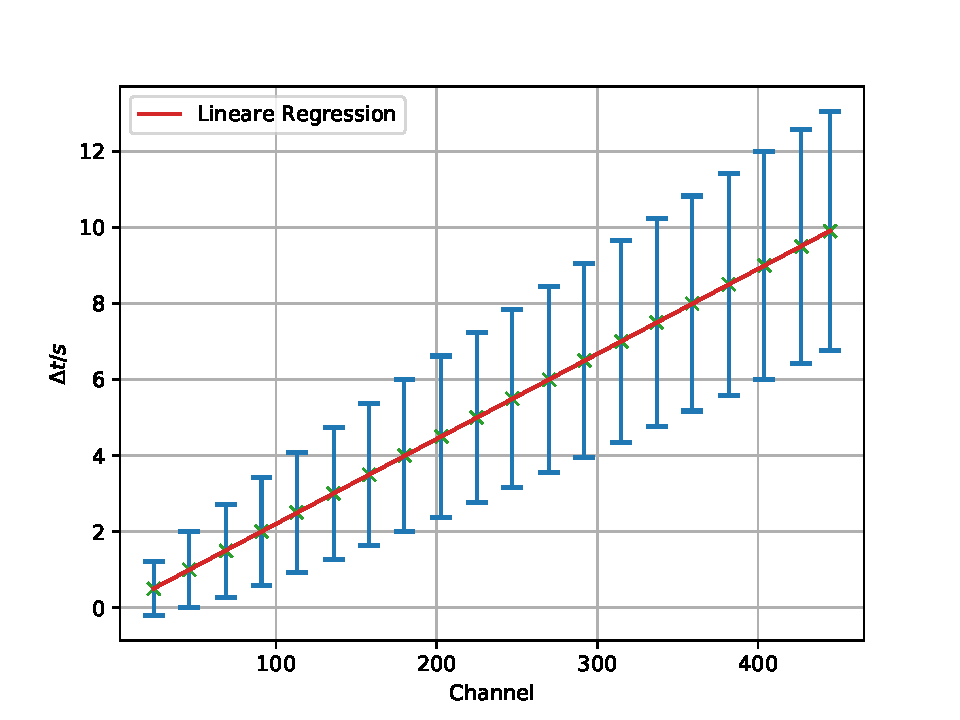
\includegraphics[width=\textwidth]{figkalibrierung.pdf}
  \caption{Kalibrierung des Multi-Channel-Analysers: Zeitlicher Abstand des Doppelimpulses $\Delta$ t gegen den zugehörigen Channel}
  \label{fig:kalibrierung}
\end{figure}
Die lineare Regression hat die Form
\begin{equation*}
  \Delta t = b \cdot C + \Delta t_{0}
\end{equation*}
und ergibt die folgenden Parameter:
\begin{align*}
  b             &=&  \SI{ 2.2341 \pm 0.0013 e-8}{\frac{s}{Channel}}  \\
  \Delta t_{0}  &=&  \SI{-3.0805 \pm 0.3453 e-8}{s}.  \\
\end{align*}
%die Parameter mit allen Nachkommastellen
%b    = 0.02234091*1e-6
%Dt0  = -0.03080493*1e-6
%db   = 1.28401232e-05*1e-6
%dDt0 = 3.45318110e-03*1e-6
Mit diesen $b$ und $\Delta t_{0}$ wird im folgenden aus dem Channel die jeweilige Lebensdauer berechnet.
\FloatBarrier

\subsection{Messung der Lebensdauer}
Die Messdaten zur Lebensdauern der Myonen sind in Abbildung \ref{fig:myonen} aufgetragen.
\begin{figure}[h!]
  \centering
  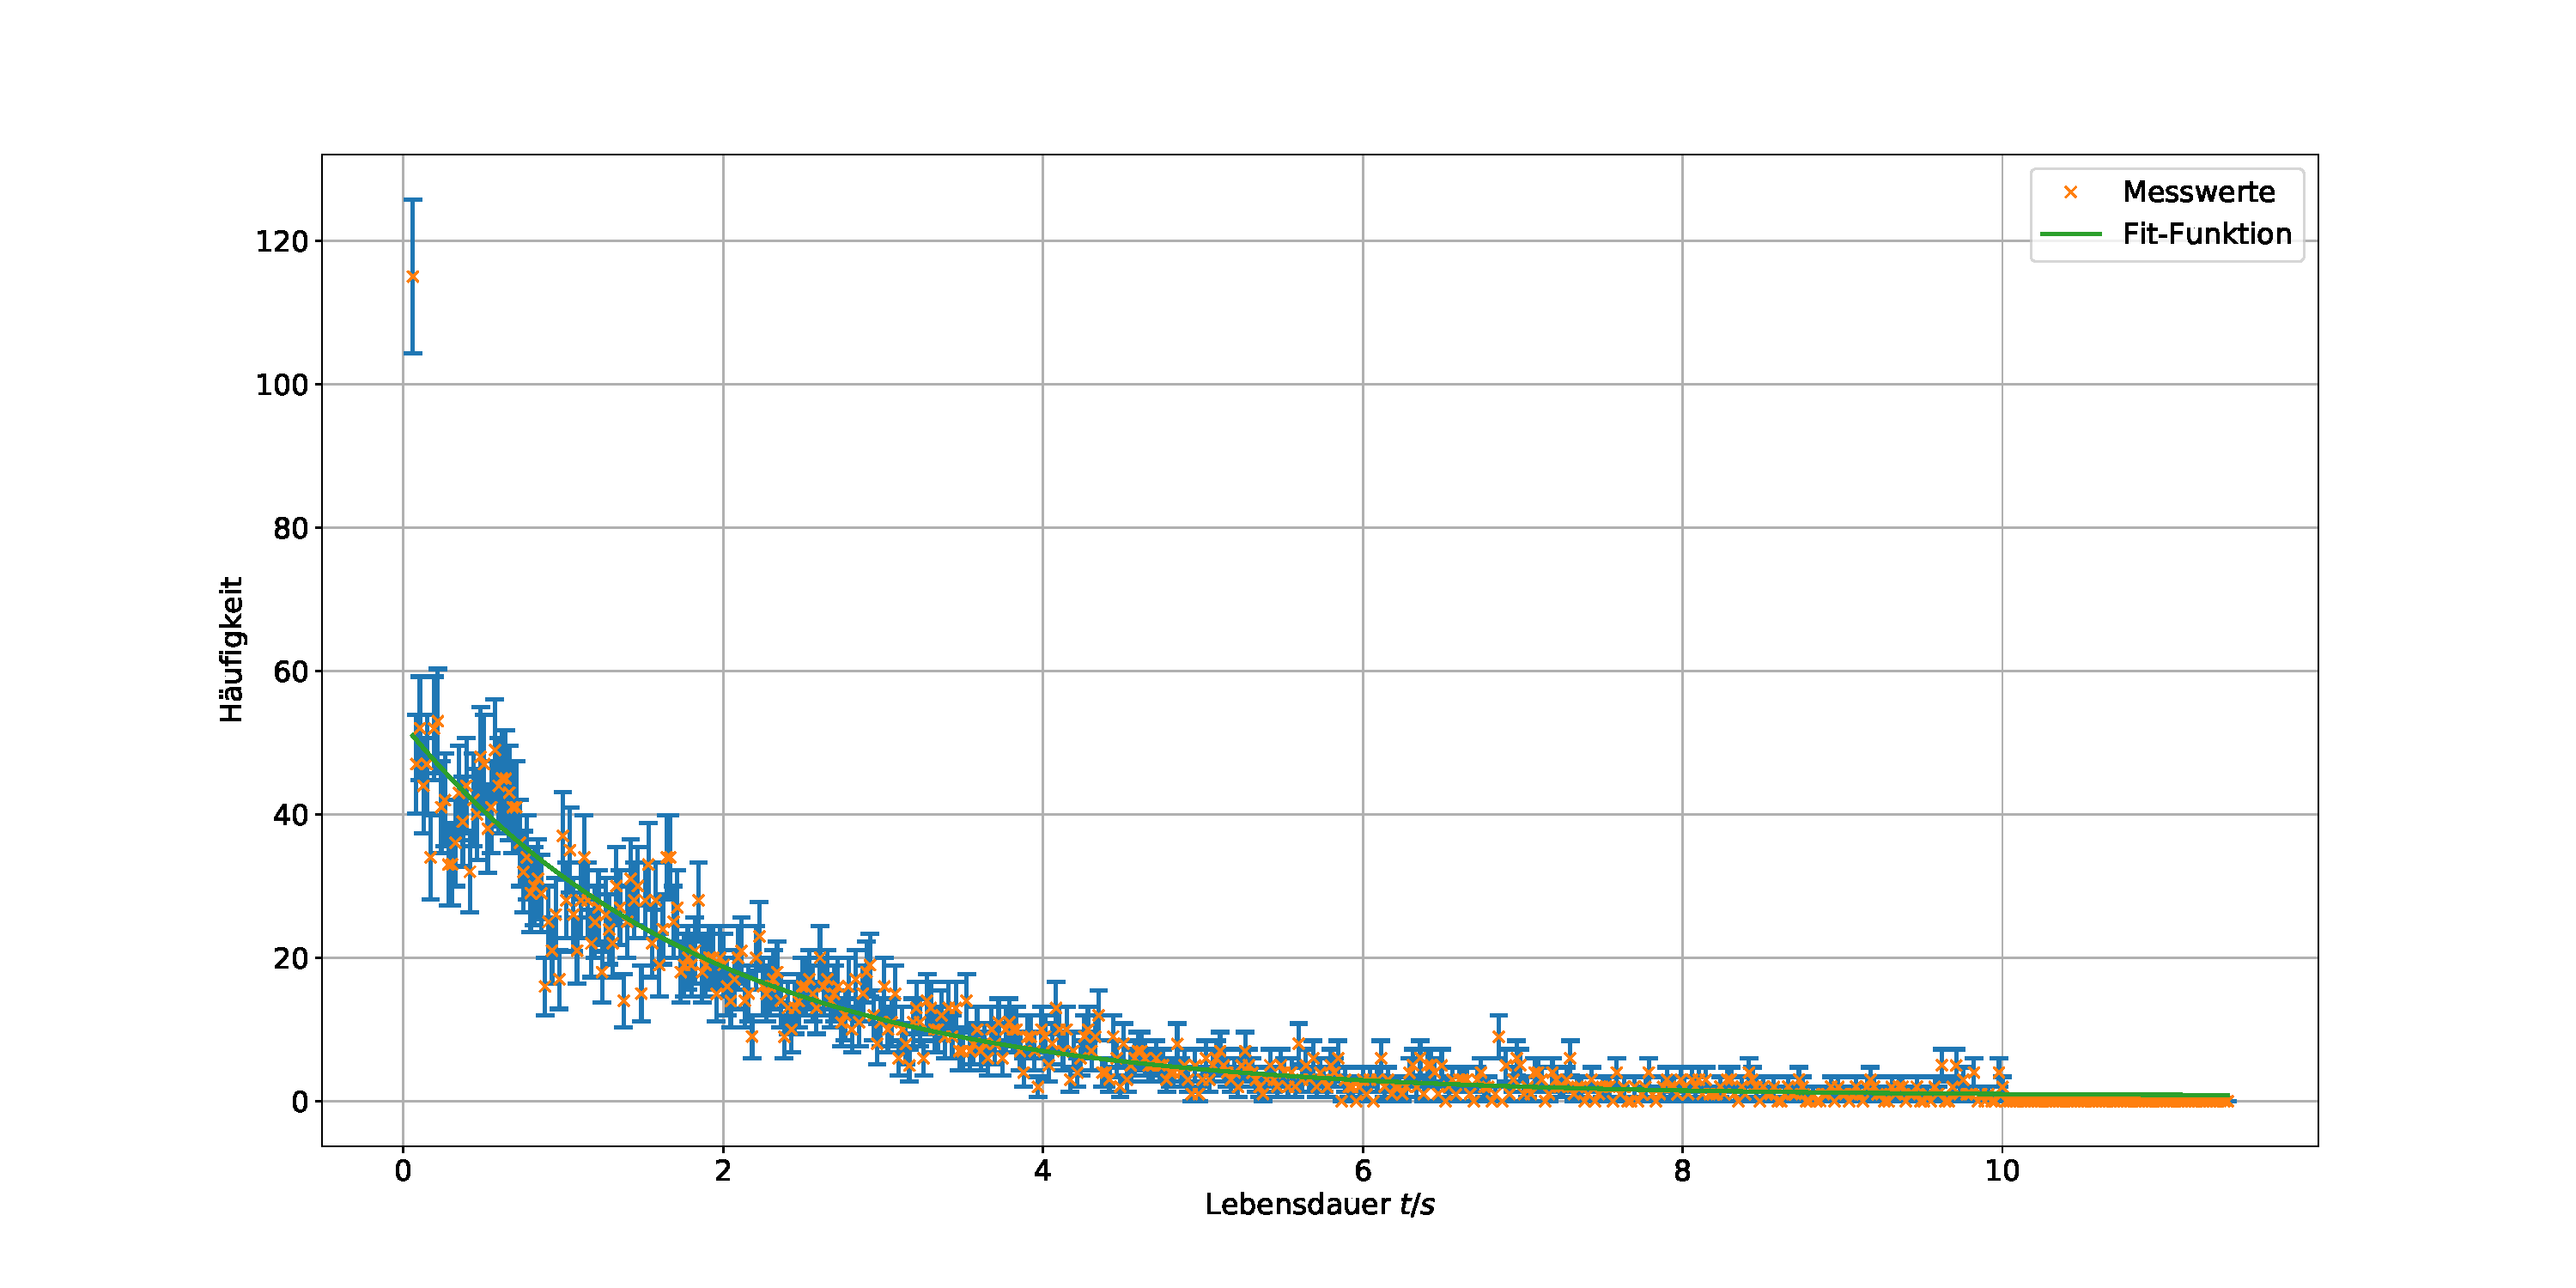
\includegraphics[width=\textwidth]{figmyonen.pdf}
  \caption{Häufigkeit der Myonenzerfälle in Abhängigkeit ihrer Lebensdauer}
  \label{fig:myonen}
\end{figure}
Die Ausgleichsrechnung der Form
\begin{equation*}
  N = N_{0} \exp{(- \lambda t)}+U_{\text{0,exp}}
\end{equation*}
bringt die Parameter
\begin{align*}
  N_{0}              &=&  \SI{51.8101 \pm 0.9677}{}\\
  \lambda            &=&  \SI{0.5282 \pm 0.01864 e06}{\frac{1}{s}}\\
  U_{\text{0,exp}}   &=&  \SI{0.7406 \pm 0.3145}{}.\\
\end{align*}
%die Parameter mit allen Nachkommastellen
%N0      = 51.81005345
%lambda  = 0.52824244
%U0      = 0.74055349
%dN0     = 0.9677403
%dlambda = 0.01864355
%dU0     = 0.31446226
Aus dem Parameter $\lambda$ wird die Lebensdauer $\tau$ bestimmt:
\begin{equation*}
  \tau_{\text{exp}}=\frac{1}{\lambda}=\SI{1.8932e-06}{s}.
\end{equation*}
Der Parameter $U_{0,exp}$ entspricht der gemessenen Untergrundrate.
Die Untergrundrate wird auch auf anderem Weg berechnet.
Hier werden weitere Größen der Messung benötigt:
\begin{align*}
  \text{Gesamte Messzeit}  && T_{\text{G}}      &=\SI{73966}{s} \\
  \text{Suchzeit}          && T_{\text{S}}      &=\SI{10e-6}{s} \\
  \text{Zählrate Start}    && N_{\text{Start}}  &=\SI{1397196}{} \\
  \text{Zählrate Stop}     && N_{\text{Stop}}   &=\SI{4719}{} \\
\end{align*}
Hierzu wird berechnet, wie viele Myonen $N_{\text{S}}$ pro Suchzeit $T_{\text{S}}$ in die Apparatur kommen. Der Fehler wird als Poissonfehler berechnet.
\begin{equation*}
  N_{\text{S}} = T_{\text{S}}\frac{N_{\text{Start}} \pm \sqrt{ N_{\text{Start}}} }{T_{\text{G}}} = \SI{0.00018889706081172433 \pm 0.000137439827129}{}.
\end{equation*}
Mit dieser Zählrate wird die Wahrscheinlichkeit $P$ berechnet, dass sich genau ein Myon in der Apparatur befindet.
\begin{equation*}
  P(1) = N_{\text{S}} \exp{(-N_{\text{S}})} = \SI{0.000188861382082 \pm 0.000137426846752}{}.
\end{equation*}
Die Untergrundrate berechnet sich dann mit der Anzahl der einbezogenen Channel $C=\SI{508}{}$ durch
\begin{equation*}
  U_{\text{0,theo}}= P(1) \frac{ N_{\text{Start}} \pm \sqrt{ N_{\text{Start}} }}{C} = \SI{0.5194416685028387 \pm 0.227912629861}{}.
\end{equation*}
%die letzten drei Werte mit allen Nachkommastellen
%NS  = 0.00018889706081172433
%P   = 0.000188861382082
%U   = 0.5194416685028387
%Fehler nacn normalem Poissonfehler
%dNS = 0.0137439827129
%dP  = 0.0137426846752
%dU  = 0.720723017881
%Fehler nach abgewandeltem Poissonfehler
%dNS = 0.000137439827129
%dP  = 0.000137426846752
%dU  = 0.227912629861
\FloatBarrier
